\documentclass{beamer} \usetheme{Madrid}
\usecolortheme{beaver}

\setbeamertemplate{enumerate items}[circle]
\setbeamercolor{item projected}{bg=red!70!black}

\usepackage[utf8]{inputenc}
\usepackage{mdframed}
\usepackage{minted}
\usepackage{tikz}
\usetikzlibrary{automata, positioning, arrows}

\tikzset{
    ->,
    node distance=3cm,
    every state/.style={thick, fill=gray!10},
    initial text=$ $,
}

\newenvironment{question}[1][]{
    \ifstrempty{#1}{}
    {\mdfsetup{
        frametitle={
            \tikz[baseline=(current bounding box.east),outer sep=0pt]
            \node[anchor=east,rectangle,fill=gray!30]
            {#1};
        }
    }}
    \mdfsetup{
        innertopmargin=10pt,linecolor=gray!30,
        linewidth=2pt,topline=true,
        frametitleaboveskip=\dimexpr - \ht\strutbox\relax
    }
    \begin{mdframed}
}{
    \end{mdframed}
}

\title{Git Workshop}
\subtitle{Fall 2020}

\author[]{Jack Leightcap\inst{1}\inst{2} \and Connor Northway\inst{2}}

\institute[IEEE, Wireless Club]{
    \inst{1}IEEE -- \url{nuieeeofficers@gmail.com}
    \and
    \inst{2}Wireless Club -- \url{nuwirelessclub@gmail.com}
}

\date[Fall 2020]{December 7, 2020}

\begin{document}
\frame{\titlepage}

\begin{frame}
    \frametitle{Intro: Workshop Structure}
    \centering \textbf{Structure:}
    \begin{enumerate}
        \setlength\itemsep{1em}
        \item Background: how does \texttt{Git} work?
        \item Example: managing homework
        \item Example: larger project
        \item Hands-on: solve \texttt{Git} `puzzles' in browser
    \end{enumerate}
    \vfill
    \centering \textbf{General:}
    \begin{itemize}
        \setlength\itemsep{1em}
        \item Ask questions!
              (want to know more? something isn't clear?)
        \item Reach out: \url{neuwireless.slack.com}
    \end{itemize}
\end{frame}

\begin{frame}
    \frametitle{Intro: Teaching \texttt{Git}}
    \begin{figure}
        
\includegraphics[height=\textheight-25mm]{xkcd.png}
        \caption{XKCD 1597 `Git' --- CC BY-NC 2.5}
    \end{figure}
\end{frame}

\begin{frame}
    \frametitle{Background: What is \texttt{Git}?}
    \vfill
    \begin{figure}
        
\includegraphics[height=15mm]{logo.png}
        \caption{Git Logo --- CC BY 3.0}
    \end{figure}
    \vfill
    \begin{itemize}
        \item broadly; \emph{a tool used to track changes to files and folders.}
        \item facilitates collaboration on software projects
        \item captures `snapshots' of a project
        \item maintains metadata
        \begin{itemize}
            \item what was changed
            \item who was it changed by
            \item when was it changed
            \item messages associated with changes
        \end{itemize}
    \end{itemize}
    \vfill
\end{frame}

\begin{frame}
    \frametitle{Background: What is \texttt{Git} used for?}
    \vfill
    \centering \textbf{Group Applications (Industry, co-op)}
    \begin{itemize}
        \item large software projects
        \item resolve conflicts when multiple people are editing the same things
        \item who wrote this!?
    \end{itemize}
    \vfill
    \centering \textbf{Personal Applications}
    \begin{itemize}
        \item ``I swear this worked 10 minutes ago\ldots''
        \item find what broke something and when
        \item separate tasks; work on bug fixing is isolated from work on new feature
        \item can use for class work!
    \end{itemize}
    \vfill
\end{frame}

\begin{frame}
    \frametitle{Background: Big Idea of \texttt{Git}}
    \begin{question}[QUESTION: Intuition]
        based on this description of what \texttt{Git} does, can you imagine how you would go about making these `snapshots' manually?
    \end{question}
    \vfill
    \begin{figure}
        
\includegraphics[width=3cm]{final.png}
    \end{figure}
\end{frame}

\begin{frame}
    \frametitle{Background: Big Idea of \texttt{Git}}
    \begin{center}
        \begin{figure}
            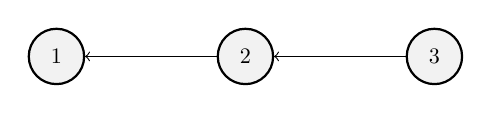
\begin{tikzpicture}[scale=0.8, every node/.style={transform shape}]
                \node[state] (q1) {1};
                \node[state, right of=q1] (q2) {2};
                \node[state, right of=q2] (q3) {3};

                \draw (q2) edge node{} (q1)
                      (q3) edge node{} (q2)
                ;
            \end{tikzpicture}
            \caption{Linear History}
        \end{figure}
        \vfill
        \begin{figure}
            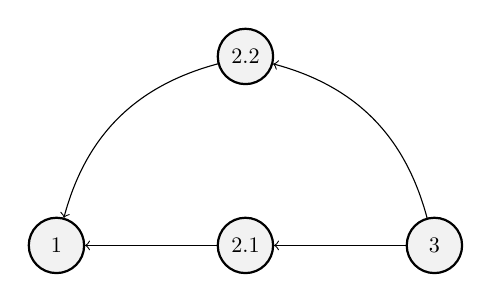
\begin{tikzpicture}[scale=0.8, every node/.style={transform shape}]
                \node[state] (q1) {1};
                \node[state, right of=q1] (q21) {2.1};
                \node[state, above of=q21] (q22) {2.2};
                \node[state, right of=q21] (q3) {3};

                \draw (q21)  edge node{} (q1)
                      (q22)  edge[bend right] node{} (q1)
                      (q3) edge node{} (q21)
                      (q3) edge[bend right] node{} (q22)
                ;
            \end{tikzpicture}
            \caption{Branched History}
        \end{figure}
    \end{center}
\end{frame}

\begin{frame}
    \frametitle{Example: Managing Local Files}
    \vfill
    \begin{question}[EXAMPLE: Homework Files]
        \begin{enumerate}
            \item \emph{Init}: make a file
            \item \emph{Add/Commit}: save file
            \item \emph{Branch/Checkout}: two new features
            \item \emph{Merge}: combine those new features
            \item \emph{Restore/Checkout}: restore save
        \end{enumerate}
    \end{question}
    \vfill
\end{frame}

\begin{frame} \frametitle{Background: \texttt{Git} vs. \texttt{GitHub}?}
    \centering \textbf{What's the difference between \texttt{Git} and \texttt{GitHub}?}
    \vfill
    \begin{columns}[t]
        \begin{column}{{\textwidth}/3}
                \centering \textbf{Git}
            \begin{itemize}
                \item tool independent of GitHub
                \item provides interface for services like GitHub
            \end{itemize}
        \end{column}
        \begin{column}{{\textwidth}/3*2}
            \centering \textbf{GitHub}
            \begin{itemize}
                \item centralized location to store git repositories
                \item alternatives: GitLab, SourceHut, BitBucket, self hosting, \ldots
                \item additional project management utilities
                \item CI, CD, hosting, \ldots
            \end{itemize}
        \end{column}
    \end{columns}
\end{frame}

\begin{frame}
    \frametitle{Example: Large Project}
    \begin{question}[EXAMPLE: Larger Project]
        \begin{itemize}
            \item Development workflow
            \item More complex histories
        \end{itemize}
    \end{question}
\end{frame}

\begin{frame}
    \frametitle{Hands-On: \texttt{learngitbranching}}
    \begin{question}[HANDS-ON: \texttt{learngitbranching}]
        \centering \url{https://learngitbranching.js.org/}
    \end{question}
\end{frame}

% connor's branching example spam
\begin{frame}
    \begin{figure}
        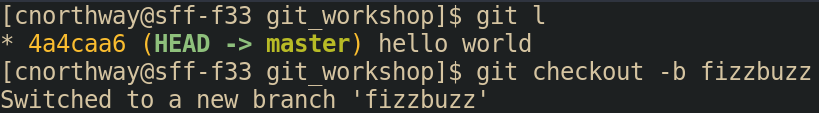
\includegraphics[height=\textwidth-2cm]{ex_imgs/1.png}
        \caption{Create and checkout 'fizzbuzz' feature branch}
    \end{figure}
\end{frame}
\begin{frame}
    \begin{figure}
        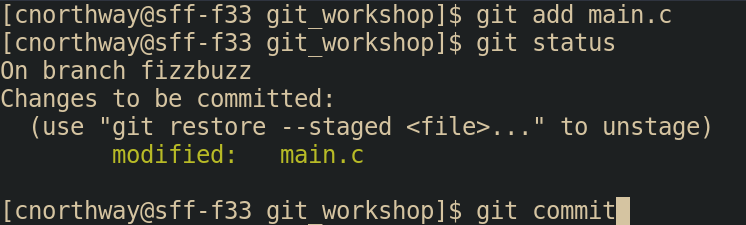
\includegraphics[height=\textwidth-2cm]{ex_imgs/2.png}
        \caption{Make some commits}
    \end{figure}
\end{frame}
\begin{frame}
    \begin{figure}
        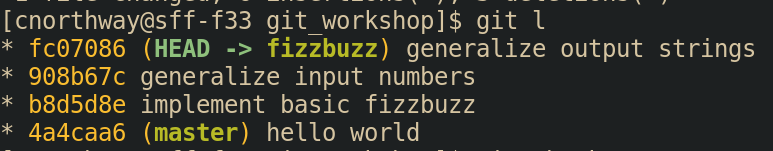
\includegraphics[height=\textwidth-2cm]{ex_imgs/3.png}
        \caption{Commits on feature branch, no other branches}
    \end{figure}
\end{frame}
\begin{frame}
    \begin{figure}
        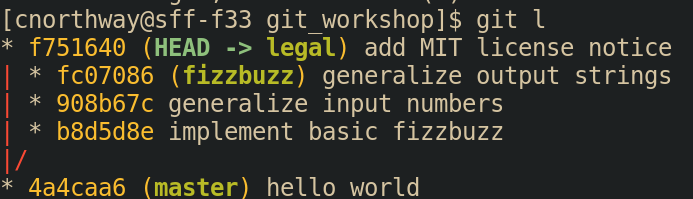
\includegraphics[height=\textwidth-2cm]{ex_imgs/4.png}
        \caption{Legal team makes new branch from master, makes changes}
    \end{figure}
\end{frame}
\begin{frame}
    \begin{figure}
        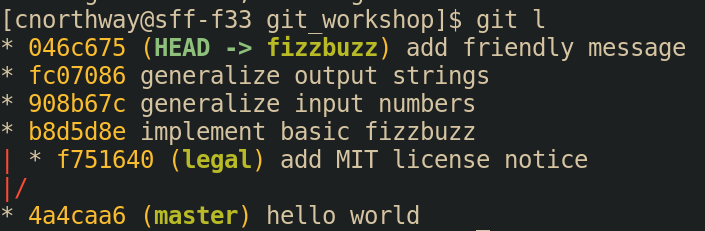
\includegraphics[height=\textwidth-2cm]{ex_imgs/5.png}
        \caption{We add another commit}
    \end{figure}
\end{frame}
\begin{frame}
    \begin{figure}
        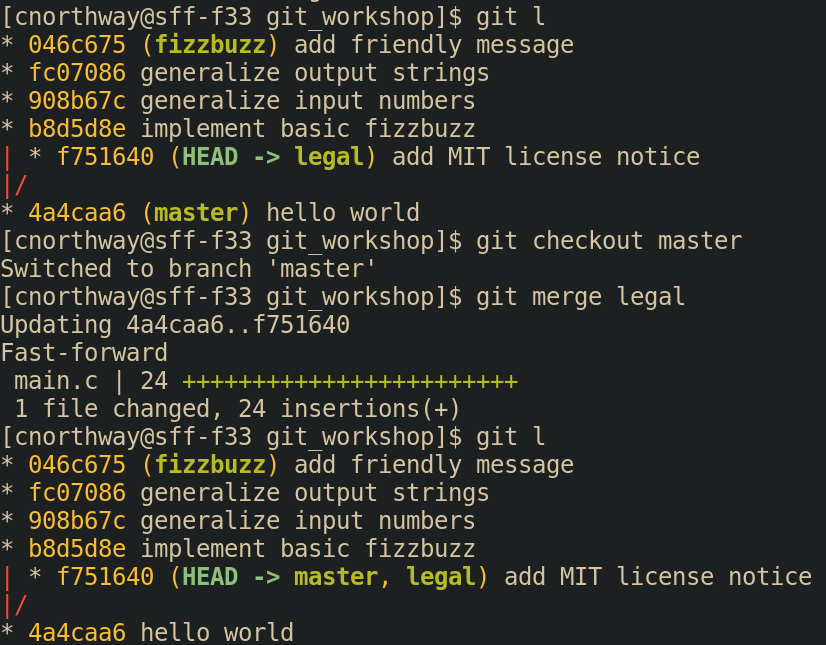
\includegraphics[height=\textwidth-2cm]{ex_imgs/6.png}
        \caption{Merge legal change to master}
    \end{figure}
\end{frame}
\begin{frame}
    \begin{figure}
        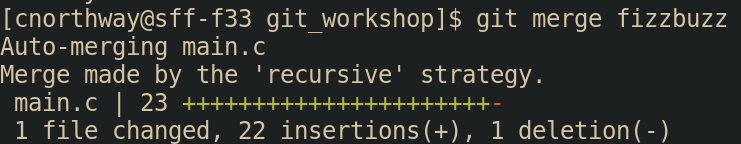
\includegraphics[height=\textwidth-2cm]{ex_imgs/7.png}
        \caption{Merge fizzbuzz -- lucky, no conflicts!}
    \end{figure}
\end{frame}
\begin{frame}
    \begin{figure}
        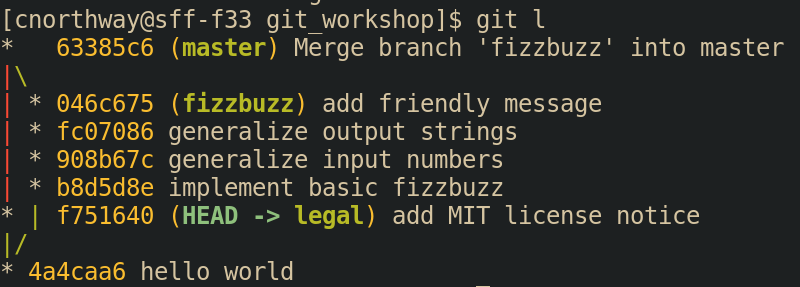
\includegraphics[height=\textwidth-2cm]{ex_imgs/8.png}
        \caption{Result of merging fizzbuzz -- merge commit with two parents}
    \end{figure}
\end{frame}

\begin{frame}
    \frametitle{See Also}
    \centering \textbf{General}
    \begin{itemize}
        \setlength\itemsep{1em}
        \item \href{https://missing.csail.mit.edu/2020/version-control/}{MIT Missing Semester Lecture 6: Version Control (Git)}
        \item \href{https://tbaggery.com/2008/04/19/a-note-about-git-commit-messages.html}{Tim Pope: A Note About Git Commit Messages}
        \item \href{https://wyag.thb.lt/}{Implement git from scratch in Python}
        \item
            \href{https://docs.github.com/en/free-pro-team@latest/github/collaborating-with-issues-and-pull-requests/about-pull-requests}{How to contribute to code on GitHub}
    \end{itemize}
    \vfill
    \centering \textbf{Git Documentation}
    \begin{itemize}
        \item \href{https://git-scm.com/docs/git-config}{Git configuration documentation}
        \item \href{https://git-scm.com/docs/gitignore}{\texttt{.gitignore} documentation}
    \end{itemize}
\end{frame}


\end{document}
